% Complejos simpliciales - Símplices y su ensamblaje
% Compilar con: pdflatex simplicial_complex.tex
\documentclass[tikz,border=10pt]{standalone}
\usepackage{tikz}
\usepackage{amsmath,amssymb}
\usetikzlibrary{arrows.meta, positioning, calc}

\definecolor{gdlblue}{RGB}{41, 98, 168}
\definecolor{gdlred}{RGB}{191, 49, 49}
\definecolor{gdlgreen}{RGB}{30, 130, 76}
\definecolor{gdlorange}{RGB}{217, 130, 30}
\definecolor{gdlpurple}{RGB}{118, 56, 138}
\definecolor{gdlgray}{RGB}{140, 140, 140}
\definecolor{gdlyellow}{RGB}{190, 140, 10}

\begin{document}
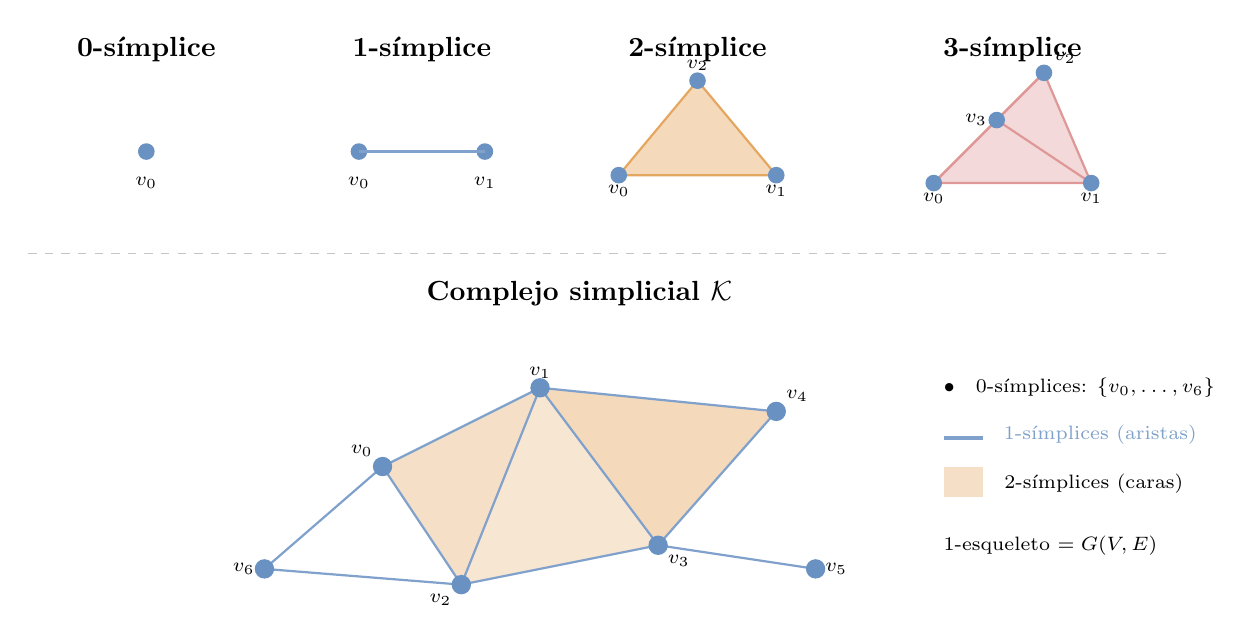
\begin{tikzpicture}[>=Stealth, font=\small]

% --- Fila superior: símplices individuales ---
\node[font=\bfseries] at (-5, 3.8) {0-símplice};
\node[font=\bfseries] at (-1.5, 3.8) {1-símplice};
\node[font=\bfseries] at (2, 3.8) {2-símplice};
\node[font=\bfseries] at (6, 3.8) {3-símplice};

% 0-símplice (punto)
\fill[gdlblue!70] (-5, 2.5) circle (3pt);
\node[below, font=\scriptsize] at (-5, 2.3) {$v_0$};

% 1-símplice (arista)
\fill[gdlblue!70] (-2.3, 2.5) circle (3pt);
\fill[gdlblue!70] (-0.7, 2.5) circle (3pt);
\draw[thick, gdlblue!60] (-2.3, 2.5) -- (-0.7, 2.5);
\node[below, font=\scriptsize] at (-2.3, 2.3) {$v_0$};
\node[below, font=\scriptsize] at (-0.7, 2.3) {$v_1$};

% 2-símplice (triángulo relleno)
\coordinate (t0) at (1, 2.2);
\coordinate (t1) at (3, 2.2);
\coordinate (t2) at (2, 3.4);
\fill[gdlorange!30] (t0) -- (t1) -- (t2) -- cycle;
\draw[thick, gdlorange!70] (t0) -- (t1) -- (t2) -- cycle;
\fill[gdlblue!70] (t0) circle (3pt);
\fill[gdlblue!70] (t1) circle (3pt);
\fill[gdlblue!70] (t2) circle (3pt);
\node[below, font=\scriptsize] at (t0) {$v_0$};
\node[below, font=\scriptsize] at (t1) {$v_1$};
\node[above, font=\scriptsize] at (t2) {$v_2$};

% 3-símplice (tetraedro)
\coordinate (s0) at (5, 2.1);
\coordinate (s1) at (7, 2.1);
\coordinate (s2) at (6.4, 3.5);
\coordinate (s3) at (5.8, 2.9);
% Caras traseras (más claras)
\fill[gdlred!15, opacity=0.5] (s0) -- (s1) -- (s3) -- cycle;
\fill[gdlred!18, opacity=0.5] (s0) -- (s2) -- (s3) -- cycle;
% Caras frontales
\fill[gdlred!25, opacity=0.6] (s0) -- (s1) -- (s2) -- cycle;
\fill[gdlred!20, opacity=0.6] (s1) -- (s2) -- (s3) -- cycle;
% Aristas
\draw[thick, gdlred!50] (s0) -- (s1) -- (s2) -- cycle;
\draw[thick, gdlred!50] (s0) -- (s3);
\draw[thick, gdlred!50] (s1) -- (s3);
\draw[thick, gdlred!50] (s2) -- (s3);
% Vértices
\fill[gdlblue!70] (s0) circle (3pt);
\fill[gdlblue!70] (s1) circle (3pt);
\fill[gdlblue!70] (s2) circle (3pt);
\fill[gdlblue!70] (s3) circle (3pt);
\node[below, font=\scriptsize] at (s0) {$v_0$};
\node[below, font=\scriptsize] at (s1) {$v_1$};
\node[above right, font=\scriptsize] at (s2) {$v_2$};
\node[left, font=\scriptsize] at (s3) {$v_3$};

% --- Separador ---
\draw[dashed, gdlgray!50] (-6.5, 1.2) -- (8, 1.2);
\node[font=\bfseries] at (0.5, 0.7) {Complejo simplicial $\mathcal{K}$};

% --- Fila inferior: complejo simplicial ensamblado ---
% Vértices del complejo
\coordinate (a) at (-2, -1.5);
\coordinate (b) at (0, -0.5);
\coordinate (c) at (-1, -3);
\coordinate (d) at (1.5, -2.5);
\coordinate (e) at (3, -0.8);
\coordinate (f) at (3.5, -2.8);
\coordinate (g) at (-3.5, -2.8);

% 2-símplices (triángulos rellenos)
\fill[gdlorange!25] (a) -- (b) -- (c) -- cycle;
\fill[gdlorange!20] (b) -- (c) -- (d) -- cycle;
\fill[gdlorange!30] (b) -- (d) -- (e) -- cycle;

% 1-símplices (aristas)
\draw[thick, gdlblue!60] (a) -- (b);
\draw[thick, gdlblue!60] (b) -- (c);
\draw[thick, gdlblue!60] (a) -- (c);
\draw[thick, gdlblue!60] (c) -- (d);
\draw[thick, gdlblue!60] (b) -- (d);
\draw[thick, gdlblue!60] (b) -- (e);
\draw[thick, gdlblue!60] (d) -- (e);
\draw[thick, gdlblue!60] (d) -- (f);
\draw[thick, gdlblue!60] (a) -- (g);
\draw[thick, gdlblue!60] (c) -- (g);

% 0-símplices (vértices)
\foreach \p/\name in {a/$v_0$, b/$v_1$, c/$v_2$, d/$v_3$, e/$v_4$, f/$v_5$, g/$v_6$} {
    \fill[gdlblue!70] (\p) circle (3.5pt);
}
\node[above left, font=\scriptsize] at (a) {$v_0$};
\node[above, font=\scriptsize] at (b) {$v_1$};
\node[below left, font=\scriptsize] at (c) {$v_2$};
\node[below right, font=\scriptsize] at (d) {$v_3$};
\node[above right, font=\scriptsize] at (e) {$v_4$};
\node[right, font=\scriptsize] at (f) {$v_5$};
\node[left, font=\scriptsize] at (g) {$v_6$};

% Leyenda
\node[anchor=west, font=\scriptsize] at (5, -0.5) {$\bullet$ \; 0-símplices: $\{v_0, \ldots, v_6\}$};
\node[anchor=west, font=\scriptsize, gdlblue!60] at (5, -1.1) {\rule{0.5cm}{1.5pt} \; 1-símplices (aristas)};
\node[anchor=west, font=\scriptsize] at (5, -1.7) {\colorbox{gdlorange!25}{\phantom{ab}} \; 2-símplices (caras)};
\node[anchor=west, font=\scriptsize] at (5, -2.5) {1-esqueleto $= G(V,E)$};

\end{tikzpicture}
\end{document}
